\documentclass{article}
\usepackage{amsmath}

\title{CS 250 Course Study Guide}
\author{Sarna Gomasta, Kyla Levin, Alexander Yeung}
\date{Fall 2023}

\usepackage[letterpaper, portrait, margin=1in]{geometry}
\usepackage{graphicx}
\usepackage{enumitem}
\usepackage{ulem}
\usepackage{amssymb}
\usepackage{amsmath}
\usepackage{tikz}

\begin{document}

\maketitle

\section*{Chapter 1: Sets and Predicate Logic}
This section has the following learning objectives:
\begin{enumerate}
    \item Translate statements to and from propositional logic
    \item Prove statements of propositional logic using truth tables and/or propositional proof rules.
    \item Translate statements to and from predicate logic.
    \item Prove statements of predicate logic using the four quantifier proof rules.
    \item Know and work with the definitions of relations (partial orders and equivalence relations) and properties of functions (one-to-one, onto, bijective).
\end{enumerate}
\subsection*{Q1.1}
Solve the following syllogism. Report the answer as a logical implication, as well as a naturally-spoken English sentence.
\begin{itemize}
    \item The only foods that my doctor recommends are ones that aren't very sweet.
    \item Nothing that agrees with me is good for dinner.
    \item Cake is always very sweet.
    \item My doctor recommends all foods that are good for dinner.
\end{itemize}
\newpage
\subsection*{Answer}
We will use the following variables: $D=\text{doctor recommends it},S=\text{sweet},A=\text{agrees with me},G=\text{good for dinner}$
\begin{itemize}
    \item This can be read as "If my doctor recommends it, then it's not very sweet." $D\rightarrow \neg S$
    \item This can be read as "There is nothing such that if it agrees with me, then it's good for dinner." $A\rightarrow G$
    \item This can be read as "If it's cake, then it's very sweet." $C\rightarrow S$
    \item This can be read as "If it's good for dinner, then my doctor recommends it." $G\rightarrow D$
\end{itemize}
$C\rightarrow S\rightarrow \neg D\rightarrow\neg G$
\\ Transitively, $C\rightarrow\neg G$
\\ In English, "If it's cake, then it's not good for dinner." Or, more naturally, "Cake is not good for dinner."
\newpage
\subsection*{Q1.2}
\begin{enumerate}[label=\alph*.]
    \item What values of $a$ and $b$ make the following statement true? Prove using a truth table.
    $$(a \lor \neg b) \land (b \land \neg a)$$
    \item What values of $a$, $b$, and $c$ make the following statement true? Prove without using a truth table.
    $$(a \lor \neg b) \land (b \land \neg a)\rightarrow (\neg c\land(a \lor b))$$
\end{enumerate}
\newpage
\subsection*{1.2 Answer}
\begin{enumerate}[label=\alph*.]
    \item What values of $a$ and $b$ make the following statement true? Prove using a truth table.
    $$(a \lor \neg b) \land (b \land \neg a)$$
    \begin{tabular}{|c|c|c|c|c|c|c|}
     \hline
     $a$ & $b$ & $\neg a$ & $\neg b$ & $(a\lor \neg b)$ & $(b\land\neg a)$ & $(a\lor \neg b)\land(b\land\neg a)$ \\ 
     \hline
     T & T & F & F & T & F & F \\  
     T & F & F & T & T & F & F \\
     F & T & T & F & F & T & F \\  
     F & F & T & T & T & F & F \\
     \hline
    \end{tabular}
    \\ To fill in the truth table, begin with the primitive values $a$ and $b$ in the leftmost columns. From there, use those values to fill in the successive $\neg a$ and $\neg b$ values in the next two columns. Continue rightways, adding columns with increasingly complex expressions using the truth values from the simpler columns until you have constructed the final expression.
    \\ As a reminder, for the binary operator "OR" ($\lor$), \textit{at least one} of the input needs to be true. For the binary operator "AND" ($\land$), \textit{both} of the input need to be true. And the unary operator "NOT" ($\neg$) will flip the truth value of its input.
    \\ As seen in the final column of the truth table, there is no combination of $a$ and $b$ values that make $(a\lor \neg b)\land(b\land\neg a)$ true.
    \item What values of $a$, $b$, and $c$ make the following statement true? Prove without using a truth table.
    $$(a \lor \neg b) \land (b \land \neg a)\rightarrow (\neg c\land(a\lor b))$$
    \\ All possible values of $a$, $b$, and $c$ will make this statement true. We know from part (a) that the antecedent of the implication step is always false. There are no $a$ and $b$ values that make it true. Therefore, there is no value that the consequent could have to make the whole implication evaluate to true. If the consequent is true, then $F\rightarrow T$ evaluates to true. If the consequent is false, then $F\rightarrow F$ still evaluates to true. 
\end{enumerate}
\newpage
\subsection*{Q1.3}

Complete a deductive sequence proof based on the following propositions:
\begin{enumerate}
    \item $\lnot p \land q$
    \item $r \rightarrow p$
    \item $\lnot r \rightarrow s$
    \item $s \rightarrow t$
\end{enumerate}
Your answer should either be a conjunction of all of the variables p,q,r,s,t which enumerates their
truth values, or you may explicitly state the truth value of each variable.
\subsection*{Answer}
\begin{enumerate}
    \item Assume $\lnot p$
    \item q (Premise 1, right separation)
    \item $\lnot p \rightarrow \lnot r$ (Contrapositive of Premise 2)
    \item $\lnot r$ (Modus Ponens of Line 3)
    \item $s$ (Modus Ponens of Premise 3)
    \item $t$ (Modus Ponens of Premise 4)
\end{enumerate}

Then our final solution is $\lnot p \land q \land \lnot r \land s \land t$
\newpage
\subsection*{1.4}
Prove by contradiction that the sum of a rational number and an irrational number is irrational. Recall that a rational number is one
which can be expressed as the quotient of two integers. An irrational number is one which cannot be represented as the quotient of two integers.
You may assume that the operations addition, subtraction, and multiplication on rationals are well-defined. In other words, the sum, difference, or
product of two rationals is always rational.
\subsection*{Answer}

Assume to the contrary, $\exists s$ such that $s = r + i$ where $r \in \mathbb{Q}$, the rational numbers, and $i \notin \mathbb{Q}$, or i is irrational.
Well, then $i = s - r$. But we know that the difference between two rational numbers is always rational. Then i must be a rational number. But this is a contradiction
because we assumed i to be irrational! 
\newpage
\section*{Chapter 2: Quantifiers and Relations}
\subsection*{2.1}
Consider the set $A=\mathbb{N}$
\\ Identify whether the following relations are reflexive, antireflexive, symmetric, antisymmetric, or transitive.
\begin{itemize}
    \item $x$ relates to $y$ if and only if $x=2y$ 
    \item $x$ relates to $y$ if and only if $x\%2=y\%2$
\end{itemize}
\newpage
\subsection*{Answer}
\begin{itemize}
    \item $x$ relates to $y$ if and only if $x=2y$
    \\ This is not reflexive, because for most numbers, $x\neq 2x$. However, it is also not antireflexive, since $x=2x$ is true for $x=0$. It is not symmetric, since if $x=2y$, then $y\neq2x$. The only case when this is true is for $x=y=0$, when $x$ and $y$ are the same. Therefore, this relation is antisymmetric. It is not transitive, since if $x=2y$ and $y=2x$, then $x=4z$, which is not always equal to $2z$.
    \item $x$ relates to $y$ if and only if $x\%2=y\%2$
    \\ This is reflexive, since $x\%2=x\%2$ for all $x$. Because it is reflexive, it cannot be antireflexive. It is symmetric, since if $x\%2=y\%2$, then   $y\%2=x\%2$. It is not antisymmetric, since this can be true of different $x$ and $y$ values. It is transitive, since if $x\%2=y\%2$ and $y\%2=z\%2$, then $x\%2=z\%2$.
\end{itemize}
\newpage
\subsection*{2.2}
TODO: Function question
\subsection*{Answer}
\newpage
\section*{Chapter 3: Number Theory}
\subsection*{Q3.1 General Number Theory}
Prove that for some relatively prime $a$ and $n$, multiplying all numbers in the set $\{1,2,...,n-2,n-1\}$ by $a$ will output a permutation of $\{1,2,...,n-2,n-1\}$.
\\ Hint: There are two parts to this proof---existence and uniqueness. To show that multiplication by $a$ permutes the elements of the set, you must show that the multiplication always produces an element in the set (existence) and you must show that that element will never be repeatedly produced via multiplication by $a$ (uniqueness). Consider how these relate to modular arithmetic and modular inverses.
\newpage
\subsection*{Answer}
As stated in the hint, we must show both the existence and uniqueness of the elements from the set when multiplied by $a$.
\\ First, to prove existence, we will prove that for some relatively prime $a$ and $n$, and for some elements $b,c\in \{1,2,...,n-2,n-1\}$,  $ab=c$ (mod $n$), unless $b=0$. This is equivalent to saying that "If $ab=0$ (mod $n$), then $b=0$ (mod $n$)". Since $a$ and $n$ are relatively prime, $a$ has an inverse in mod $n$. Multiply both sides by $a^{-1}$ (mod $n$) to get $aba^{-1}=0(a^{-1})$ (mod $n$). $aa^{-1}$ will cancel out to 1, showing that $b=0$ (mod $n$).
\\ Next, to prove uniqueness, we will show that for some relatively prime $a$ and $n$, if $ab=ac$ (mod $n$), then $b=c$. Once again, because $a$ and $n$ are relatively prime, we know $a$ must have some inverse $a^{-1}$ (mod $n$). Multiplying both sides by $a^{-1}$ gives $aba^{-1}=aca^{-1}$ (mod $n$), leaving $b=c$ (mod $n$).
\\ Putting the two pieces together, we know that multiplying any element of $\{1,2,...,n-2,n-1\}$ by some constant $a$, which is relatively prime to $n$, will never result in 0 and therefore will always produce some number in the range of 1 to $n-1$. Furthermore, no multiplication will result in the same number. Therefore, the output will be a permutation of the original set $\{1,2,...,n-2,n-1\}$.
\newpage
\subsection*{Q3.2 Euclid's Algorithm}

Let $a = 473$ and $b = 47$. Run Euclid's Algorithm on a and b to find their GCD. What can you conclude about a and b from your run of Euclid's Algorithm?

\subsection*{Answer}

\begin{align*}
473 &= 10 \times 47 + 3 \\
47 &= 15 \times 3 + 2 \\
3 &= 1 \times 2 + 1 \\
2 &= 2 \times 1 + 0 \\
\end{align*}

The GCD of 473 and 47 is 1 since the algorithm ends with a remainder of 1. Since their GCD is 1, the two numbers are relatively prime.
\newpage
\subsection*{Chinese Remainder Theorem (CRT)}
\newpage
\section*{Chapter 4: Induction and Recursion}
\subsection*{4.1}
Explain the error in the following induction proof:
\\ \textbf{Claim}: All students are the same height.
\\ Base case: Consider a set of students of size 1. Any student is the same height as themselves, and so all students in the set are the same height.
\\ \textbf{Inductive hypothesis}: All students in a set of size $n$ have the same height. 
\\ \textbf{Inductive step}: Now suppose we have a set of $n+1$ students, labeled $s_1$ through $s_{n+1}$: $\{s_1,s_2,s_3,...,s_{n-1},s_n,s_{n+1}\}$.
\\ Consider the entire set of $n+1$ students as two individual sets of $n$ students each.
\\ The first set contains students $s_1$ through $s_n$: $\{s_1,s_2,s_3,...,s_{n-1},s_n\}$
\\ The second set contains students $s_2$ through $s_{n+1}$: $\{s_2,s_3,...,s_{n-1},s_n,s_{n+1}\}$
\\ Both sets contain $n$ students, and so by the inductive hypothesis, all students in each set must be of the same height. And if all students in each set have the same height, then all students in the full $n+1$ set must have the same height.
\\ In conclusion, all students in any set of size $n\geq1$ must have the same height.
\newpage
\subsection*{Answer}
The error in the proof can be attributed to the overlap between the two sets in the inductive step. The base case is easy to observe for some set $\{s_1\}$, but when the inductive step is applied to "step" from $n=1$ to $n=2$, the two sets described in the inductive step would be $\{s_1\}$ and $\{s_2\}$, in which may be two students of differing heights. So while $s_1$ and $s_2$ are the same heights as themselves, this does not mean that they are the same height as one another.
\newpage
\subsection*{4.2}
Suppose we have a recursively-defined function (much like a Fibonacci sequence) $f_n=5f_{n-1}-6f_{n-2}$ where $f_0=2$ and $f_1=5$.
\\ Prove inductively that $f_n=2^n+3^n$ for all $n\geq0$.
\subsection*{Answer}
\textbf{Claim}: $f_n=2^n+3^n$ for all $n\geq0$
\\ \textbf{Base case}: For $n=0$: $f_0=2$, and $2^0+3^0=1+1=2$. For $n=1$: $f_1=5$ and $2^1+3^1=2+3=5$.
\\ \textbf{Inductive hypothesis}: Assume that $f_n=2^n+3^n$ for all $n\geq0$
\\ \textbf{Inductive step}:
\begin{itemize}[label=]
    \item $f_{n+1}=5f_n-6f_{n-1}$
    \item $f_{n+1}=5(2^n+3^n)-6(2^{n-1}+3^{n-1})$ By inductive hypothesis
    \item $f_{n+1}=5(2^n)+5(3^n)-3(2^n)-2(3^n)$
    \item $f_{n+1}=2(2^n)+3(3^n)$
    \item $f_{n+1}=2^{n+1}+3^{n+1}$
\end{itemize}
\newpage
\section*{Chapter 9: Graphs and Trees}
\subsection*{9.1}
How many different undirected graphs with $n$ nodes are possible? Assume that two graphs with $n$ nodes are "different" if they have different edges and give your answer as an expression of $n$.
\newpage
\subsection*{Answer}
First, we must find out how many possible edges can exist in an undirected graph with $n$ nodes. This is the same as the number of edges that would be in the complete graph. There are many different ways to think about this:
\begin{itemize}
    \item Consider the adjacency matrix of the graph. Since there are $n$ nodes in the graph, the matrix is of size $n\times n$, and since the graph is complete, every entry in the matrix would be 1 except along the diagonal (since edges cannot be directed at themselves). So the number of edges would be the number of 1's in the matrix, divided by 2 so as not to double-count. This gives $\frac{(n\times n)-n}{2}$ or $\frac{n(n-1)}{2}$
    \item Number the nodes from 1 to $n$. Beginning at node 1, it can have up to $n-1$ edges with the other $n-1$ nodes. The next, up to $n-2$ edges, the next, $n-3$, and so on. This gives the sum $(n-1)+(n+2)+...+2+1$, which is also equal to $\frac{n(n-1)}{2}$ through a combinatorial proof (not covered in this class).
    \item In a complete graph, all $n$ nodes would have a degree of $n-1$. Sum this up across all nodes, and the total degree is $n(n-1)$. Then, to find the number of edges, divide by 2 to remove the duplicates, because one edge will be one degree in two separate nodes. This also gives $\frac{n(n-1)}{2}$
    \item Consider all $n$ nodes as a set. From this set, one can \textit{choose} any unordered pair of two nodes to form an edge. This is the definition of the \textit{choose} operation, and so there are $n\choose 2$ possible edges. This again is equivalent to $\frac{n(n-1)}{2}$ edges by combinatorial proof.
\end{itemize}
Now that we know that there are $\frac{n(n-1)}{2}$ possible edges, we can think of these edges as being a set of edges, and each possible graph on $n$ nodes having some subset of those edges. To figure out how many different graphs are possible, we must figure out how many possible subsets there are for a set with $\frac{n(n-1)}{2}$ edges. This is the same as finding the size of the power set of the set of edges, which is $2^{\frac{n(n-1)}{2}}$.
\newpage
\section*{Chapter 5: Regular Expressions}
\subsection*{5.1}
Assume the alphabet $\sum=\{0,1\}$. If the English description is given, provide the regular expression. If the regular expression is given, give a short, English description of the accepted set of strings.
\begin{enumerate}[label=\alph*.]
    \item The set of strings that contain at least one 0 and at least one 1.
    \item $(1+\lambda)(00^*1)^*0^*$
    \item The set of strings such that all pairs of adjacent 0's appear before any pairs of adjacent 1's.
\end{enumerate}
\newpage
\subsection*{Answer}
\begin{enumerate}[label=\alph*.]
    \item This can be thought of as either a 0 appearing before the 1, or the 1 appearing before the 0. Since these are the only mandated characters, the rest of the string can be any combination of 0's and 1's that come before, in-between, or after the 0 and 1. In other words, there are two possible string formats: $(0+1)^*0(0+1)^*1(0+1)^*$ or $(0+1)^*1(0+1)^*0(0+1)^*$
    \\ Together, the full regex is $((0+1)^*0(0+1)^*1(0+1)^*)+((0+1)^*1(0+1)^*0(0+1)^*)$
    \item The language starts with either a 1 or an empty string. From there, it is followed by a 0, some number of zero's, and then a 1. Just looking at these parts, the string can start as either:
    \\ 1 0 0... 1 
    \\ 0 0... 1
    \\ Even if the 0... is omitted, the string can only start with 0 1. 1 1 is not allowed.
    \\ Looking further, we can observe that within the $(00^*1)$ part, removing the optional 0's, $(01)$ the structure mandates that 0 must come before 1. So if this block repeats, the structure will looks like this: 0 1 0 1 with more 0's padding the in-between. And since only more 0's are added onto the end, we can conclude that this will be the set of all strings without consecutive 1's.
    \item This can be divided into two parts: The first part of the string that does not allow 11's, but does allow 00's, and the second part of the string that does not allow 00's, but does allow 11's.
    \\ For a binary string where 11 cannot occur, this could be any combination of 0's or 10's, either ending in a 1 or not: $(0+10)^*(1+\lambda)$
    \\ The formula is much the same for a binary string where 00 cannot occur: $(1+01)^*(0+\lambda)$
    \\ Concatenating the two together gives us the final string: $(0+10)^*(1+\lambda)(1+01)^*(0+\lambda)$
\end{enumerate}
\newpage
\section*{Chapter 14: Finite Automata}
\subsection*{14.1}
Assume $\sum=\{0,1\}$. Draw a DFA for the language that accepts all binary strings with either an even number of 0's or contains exactly two 1's.
\subsection*{Answer}
Let us first consider what states this machine will need. The machine considers strings based on two different criteria, although a string only needs one to be accepted. The first condition is that there is an even number of 0's. There are only two states for this, an even number of 0's or an odd number of 0's. Reading in 0's would switch between the two states like so:
\begin{center}
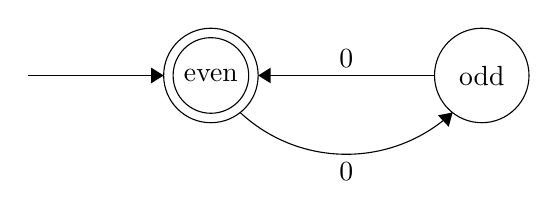
\begin{tikzpicture}[scale=0.2]
\tikzstyle{every node}+=[inner sep=0pt]
\draw [black] (26,-20.8) circle (3);
\draw (26,-20.8) node {even};
\draw [black] (26,-20.8) circle (2.4);
\draw [black] (43.2,-20.8) circle (3);
\draw (43.2,-20.8) node {odd};
\draw [black] (41.348,-23.145) arc (-46.98484:-133.01516:9.892);
\fill [black] (41.35,-23.15) -- (40.42,-23.33) -- (41.1,-24.06);
\draw (34.6,-26.3) node [below] {$0$};
\draw [black] (40.2,-20.8) -- (29,-20.8);
\fill [black] (29,-20.8) -- (29.8,-21.3) -- (29.8,-20.3);
\draw (34.6,-20.3) node [above] {$0$};
\draw [black] (14.4,-20.8) -- (23,-20.8);
\fill [black] (23,-20.8) -- (22.2,-20.3) -- (22.2,-21.3);
\end{tikzpicture}
\end{center}
Now let us consider the other criteria, which is "exactly two 1's". This has four states: zero 1's, exactly one 1, exactly two 1's, and more than two 1's, since beyond two 1's, that criteria will always fail. Reading in any 1 will move between these states, ending with the "more than two 1's" state in a dead end.
\begin{center}
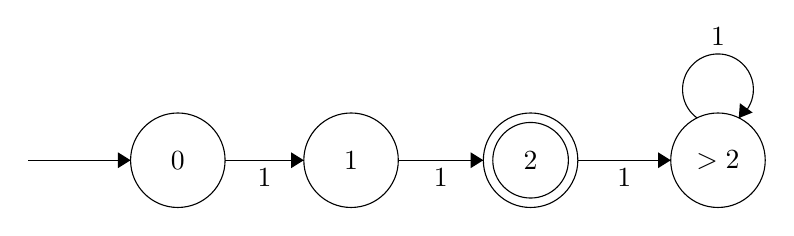
\begin{tikzpicture}[scale=0.2]
\tikzstyle{every node}+=[inner sep=0pt]
\draw [black] (28.9,-20.3) circle (3);
\draw (28.9,-20.3) node {$1$};
\draw [black] (40.3,-20.3) circle (3);
\draw (40.3,-20.3) node {$2$};
\draw [black] (40.3,-20.3) circle (2.4);
\draw [black] (52.2,-20.3) circle (3);
\draw (52.2,-20.3) node {$>2$};
\draw [black] (17.9,-20.3) circle (3);
\draw (17.9,-20.3) node {$0$};
\draw [black] (31.9,-20.3) -- (37.3,-20.3);
\fill [black] (37.3,-20.3) -- (36.5,-19.8) -- (36.5,-20.8);
\draw (34.6,-20.8) node [below] {$1$};
\draw [black] (43.3,-20.3) -- (49.2,-20.3);
\fill [black] (49.2,-20.3) -- (48.4,-19.8) -- (48.4,-20.8);
\draw (46.25,-20.8) node [below] {$1$};
\draw [black] (20.9,-20.3) -- (25.9,-20.3);
\fill [black] (25.9,-20.3) -- (25.1,-19.8) -- (25.1,-20.8);
\draw (23.4,-20.8) node [below] {$1$};
\draw [black] (8.4,-20.3) -- (14.9,-20.3);
\fill [black] (14.9,-20.3) -- (14.1,-19.8) -- (14.1,-20.8);
\draw [black] (50.877,-17.62) arc (234:-54:2.25);
\draw (52.2,-13.05) node [above] {$1$};
\fill [black] (53.52,-17.62) -- (54.4,-17.27) -- (53.59,-16.68);
\end{tikzpicture}
\end{center}
Since one criteria only cares about 0's being read in, and the other only cares about 1's being read in, we can combine the two into one machine with 8 states, each representing a state from the even/odd criteria \textit{and} a state from the "how many 1's" criteria.
\begin{center}
    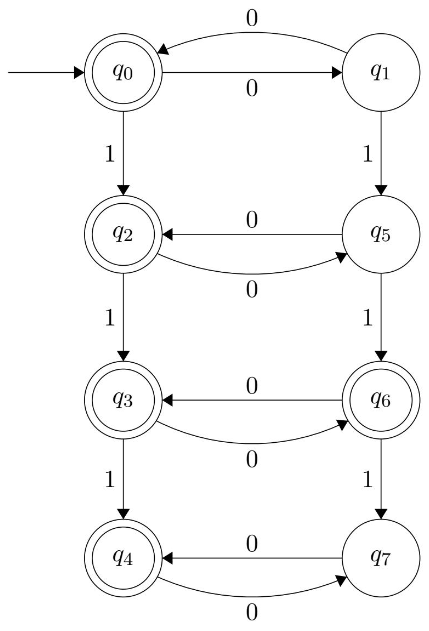
\includegraphics[width=6cm]{Screenshot 2023-11-21 143618.png}
\end{center}
\newpage
\subsection*{14.2}
TODO: DFA Simplification question
\subsection*{Answer}
\newpage
\subsection*{14.3}
TODO: DFA to NFA conversion question
\subsection*{Answer}
\newpage
\subsection{14.4}
Let $L^R$ be any arbitrary regular language. Let the language $L^R = {w^R : w \in L}$ be the reversal of L.
Show that $L^R$ is regular.
\subsection*{Answer}

Since we know that $L$ is regular, we know that there exists some DFA or equivalent NFA which accepts $L$. Without loss of generality, we can
assume that there exists only start or end state (If a DFA had multiple accepting states, you could eliminate them down to just one 
by redirecting all of the arrows going into other accepting states into a single accepting state, and eliminating the redundant accepting
states). Then we can construct a DFA or equivalent NFA which accepts $L^R$ by making the start state and accepting state, the accepting state
a start state, and reversing every state transition (reversing the "arrows"). Then we have a machine that traverses backwards over every
string in $L$, and have thus constructed a DFA for $L^R$. Since there exists a DFA / NFA for $L^R$, we know that $L^R$ is regular.
\newpage
\subsection*{14.5}
TODO: $\lambda-$NFA problem
\subsection*{Answer}
\newpage
\section*{Chapter 15: Formal Language Theory}
\subsection*{15.1}
Let L be a language that is Turing Recognizable by some Turing Machine. Let L' be the language $\Sigma^* - L$,
and let that language also be Turing Recognizable by some other Turing Machine. Prove that L is Turing Decidable.
(Hint: Recall that a single-tape Turing Machine can be used to simulate a multi-tape Turing Machine)
\subsection*{Answer}
We know this to be true by the TR / TD Theorem. But for a rigorous proof, recall that a multi-tape Turing Machine can be simulated by
a single-tape Turing Machine. Then we will construct a multi-tape Turing Machine which runs the Turing Machines for L and L' in parallel. One of these
is guaranteed to terminate, since $L + L' = \Sigma^*$. If, on any given string, the Turing Machine that recognizes L terminates, 
we know that string is in L. If the Turing Machine that recognizes L' terminates, we know that string is not in L. Then here we have
constructed a Turing Machine that always decides whether or not a string is in L, and so L is Turing Decidable.
\end{document}